\section{Evaluation framework}\label{sec:evaluation-framework}

In order to answer the research questions defined in section \ref{sec:research-question},
we have designed an evaluation framework that allows us to compare the performance of the proposed method against the state-of-the-art in the field of text classification attacks.


\subsection{Semantic preservation evaluation}\label{subsec:qualitative-evaluation}
%**************************************************************

We started evaluating the statistics of the attack processes measuring the \emph{attack metrics}.
To investigate the quality of adversarial examples, we used the \emph{quality metrics}, namely the Sentence BERT similarity, the perplexity and the contradiction rate.

Table \ref{tab:results-imdb} shows the results of the three attacks under analysis performed on the IMDB dataset.
Table \ref{tab:results-rotten} does the same for the Rotten Tomatoes dataset.

TextFooler is by far the most effective attack, since it has the highest number of successful attacks and it reaches the lowest accuracy under attack.
Whilst SynBA has a high success rate on IMDB (92.7\%), it drops to 68.56\% on Rotten Tomatoes, where the attack is more challenging due to the limited amount of words.
But still, it performs better than BAE.

Moreover, SynBA effectively attack the model by perturbing just a few words (4.95\% on IMDB and 14.05\% on Rotten Tomatoes), while TextFooler and BAE generally tend to swap more words.

Regarding the quality metrics, we can clearly see that SynBA outperforms TextFooler on both datasets. 
In particular, it is able to generate more fluent adversarial examples, since the attack perplexity is lower than the one with TextFooler. 
Although BAE has a better attack perplexity than SynBA, the latter has a significantly higher semantic similarity on Rotten Tomatoes (0.901).
The good perplexity obtained by BAE is justified by the fact that it uses a language model to generate candidates, which are more natural than those generated by SynBA.
Nevertheless, BAE has the drawback of generating adversarial examples inconsistent with the original counterpart, indeed it has a significant contradiction rate (53.6\% on IMDB and 16.4\% on Rotten Tomatoes).
Whereas SynBA successfully reduces the contradiction rate (4.9\% on IMDB, 12.3\% on Rotten Tomatoes), meaning that the adversarial samples are more likely to be consistent with the original text.

Generally speaking, those outcomes highlight that our proposed solution is able to craft high-quality adversarial examples that are able to fool the target model, while preserving the original semantics of the text and the fluency of the sentences.

\begin{table}[h]
    \footnotesize
    \centering
    \begin{tabular}{|l|c|c|c|}
        \hline
        {} &           \textbf{TextFooler} &   \textbf{BAE} &    \textbf{SynBA} \\
        \hline \hline
        \emph{Successful attacks}  ($\uparrow$)             &      \textbf{917} &             608 &               864 \\
        \emph{Failed  attacks}  ($\downarrow$)                &       \textbf{15} &             324 &                68 \\
        \emph{Skipped  attacks}  ($\downarrow$)             &       68 &              68 &                68 \\
        \emph{Original/pertuberd accuracy}  ($\downarrow$)   &     \textbf{93.2/1.5} &            93.2/32.4 &              93.2/6.8 \\
        \emph{Attack success rate}  ($\uparrow$)              &    \textbf{98.39} &           65.24 &              92.7 \\
        \emph{Avg word perturbed}  ($\downarrow$)               &     8.76 &            \textbf{4.49} &              4.95 \\
        \emph{Avg original/perturbed perplexity}  ($\downarrow$)       &    41.48/63.0 &           \textbf{41.78/48.4} &              41.5/50.74 \\
        \emph{Avg SBERT similarity} ($\uparrow$)          &    0.928 &           \textbf{0.964} &             0.944 \\
        \emph{Attack contradiction rate} ($\downarrow$)      &    0.053 &           0.164 &             \textbf{0.049} \\
        \hline
        \end{tabular}
    \caption{Attack results on IMDB dataset}
    \label{tab:results-imdb}
\end{table}

\begin{table}[h]
    \footnotesize
    \centering
    \begin{tabular}{|l|c|c|c|}
        \hline
        {} &           \textbf{TextFooler} &   \textbf{BAE} &    \textbf{SynBA} \\
        \hline \hline
        \emph{Successful attacks} ($\uparrow$)           &    \textbf{754} &   522                &         578 \\
        \emph{Failed  attacks} ($\downarrow$)              &     \textbf{89} &   321                &         265 \\
        \emph{Skipped  attacks} ($\downarrow$)            &    157 &   157                &         157 \\
        \emph{Original/pertuberd accuracy} ($\downarrow$)  &   \textbf{84.3/8.9} &  84.3/32.1       &  84.3/26.5 \\
        \emph{Attack success rate} ($\uparrow$)          &   \textbf{89.44} &     61.92  &    68.56 \\
        \emph{Avg word perturbed} ($\downarrow$)          &   19.48 &     15.07           &    \textbf{14.05} \\
        \emph{Avg original/perturbed perplexity} ($\downarrow$)    &   72.58/154.52 &     \textbf{76.96/99.91}          &    72.05/112.08 \\
        \emph{Avg SBERT similarity} ($\uparrow$)        &   0.805 &     0.776           &    \textbf{0.901} \\
        \emph{Attack contradiction rate} ($\downarrow$)    &   0.196 &     0.536           &    \textbf{0.123} \\
        \hline
        \end{tabular}

    \caption{Attack results on Rotten Tomatoes dataset}
    \label{tab:results-rotten}
\end{table}




%**************************************************************

\subsection{Cost assessment}\label{subsec:quantitative-evaluation}

For a comprehensive evaluation of the proposed method, we have also measured the execution time for each component of SynBA and compared it with the baselines.
Table \ref{tab:runtime-imdb} and \ref{tab:runtime-rotten}  show the results of the experiments respectively on IMDB and Rotten Tomatoes datasets.

A glance at the tables reveals that SynBA is the fastest attack, since it requires less time to generate the adversarial examples (on average 7.7 seconds on IMDB, 1.4 seconds on Rotten Tomatoes).
In particular, it takes advantage of the word importance ranking, which is the most time-consuming component of the attack. Indeed the gradient-based method saves us from having to make several queries to the model for each word in the sentence.
This affects also the average number of queries to the model during the whole attack, which results in a dramatically lower value for SynBA compared to the other two attacks.

As expected the SynBA transformation takes a little longer than the one of TextFooler and BAE, since it computes three different pools of candidates that then are combined together.

The only constraint that strongly impacts the runtime analysis is Sentence-BERT, and the longer the inputs, the more time it takes to compute the semantic similarity between the original and the perturbed example --- approximately 48 ms on IMDB and 15 ms on Rotten Tomatoes.

\begin{table}[h]
    \footnotesize
    \centering
    \begin{tabular}{|l||c|c|c|}
        \hline
        {} &            \textbf{TextFooler} &   \textbf{BAE} &    \textbf{SynBA} \\
        \hline \hline
        \emph{Avg attack time}  ($\downarrow$)          &      16.61 &     23.462 &     \textbf{7.686} \\
        \hline
        \emph{Avg WIR time} ($\downarrow$)        &       3.25 &      3.341 &    \textbf{0.087} \\
        \hline
        \emph{Avg transformation time} ($\downarrow$)      &      \textbf{0.147} &      0.252 &     0.191 \\
        \hline
        \emph{Avg constraints time} ($\downarrow$)   &   \textbf{0.0140}      &   0.0217       &   0.0555       \\      
        WordEmbeddingDistance        &  0.0002 &          &   0.0001 \\
        PartOfSpeech                 &  0.0065 &  0.0115  &   0.0073 \\
        UniversalSentenceEncoder     &  0.0073 &  0.0102  &          \\
        BERT                         &         &          &   0.0481 \\
        \hline
        \emph{Avg num queries} ($\downarrow$)             &    604.85 &      352.21 &     \textbf{191.14} \\
        \hline
        \end{tabular}
    \caption{Runtime analysis on IMDB dataset in seconds}
    \label{tab:runtime-imdb}
\end{table}


\begin{table}[h]
    \footnotesize
    \centering
    \begin{tabular}{|l||c|c|c|}
        \hline
        {} &            \textbf{TextFooler} &   \textbf{BAE} &    \textbf{SynBA} \\
        \hline \hline
        \emph{Avg attack time} ($\downarrow$)            &  2.049 &   1.578 &   \textbf{1.439} \\
        \hline
        \emph{Avg WIR time} ($\downarrow$)               &  0.189 &   0.189 &  \textbf{0.083} \\
        \hline
        \emph{Avg transformation time} ($\downarrow$)    &  \textbf{0.011} &   0.073 &   0.105 \\
        \hline
        \emph{Avg constraints time} ($\downarrow$)       &  \textbf{0.0116}       &  0.0195        &   0.0226       \\
        WordEmbeddingDistance        &  0.0002 &          &   0.0001 \\
        PartOfSpeech                 &  0.0057 &  0.0111  &   0.0069 \\
        UniversalSentenceEncoder     &  0.0058 &  0.0084  &          \\
        BERT                         &         &          &   0.0156 \\
        \hline
        \emph{Avg num queries} ($\downarrow$)            &  110.15 &    56.77 &    \textbf{45.27} \\
        \hline
        \end{tabular}
    \caption{Runtime analysis on Rotten Tomatoes dataset in seconds}
    \label{tab:runtime-rotten}
\end{table}



\subsection{Human evaluation}\label{subsec:human-evaluation}

Up to now, we have evaluated the proposed method in terms of \emph{semantic similarity} and \emph{language fluency} using automatic metrics.
We still have to accomplish one of three utility-preserving properties described in section \ref{sec:defined-goal}: \emph{human prediction consistency}.

The only way to measure this property is to ask human annotators to evaluate the generated adversarial examples.

We sampled 100 successful adversarial examples from the results obtained with TextFooler, BAE and SynBA on the Rotten Tomatoes dataset.
We ask three human annotators to evaluate each set of 100 pairs (original and perturbed sample).
The task is to decide if the perturbed sample is consistent with the original one, meaning that the label predicted by human judges on the input and the adversary should be the same.
Language fluency and grammatical or spelling errors are not considered in this task.

During the survey, participants were asked to rate the sample pairs with one of the following three annotation labels: 
\begin{itemize}
    \item \textbf{Consistent}: the perturbed sample is consistent with the original one.
    \item \textbf{Inconsistent}: the perturbed sample is not consistent with the original one.
    \item \textbf{Unclear}: the perturbed sample is not clear enough to be evaluated.
\end{itemize}


A Jupyter notebook has been developed to collect the annotations. In particular, we use \texttt{pigeon}\footnote{\url{https://github.com/agermanidis/pigeon}}, a python library to easily annotate each adversarial sample one by one according to the consistency perceived.
An example of the interface used by human judges is shown in Figure \ref{fig:human-evaluation-form}.

\begin{figure}
    \centering
    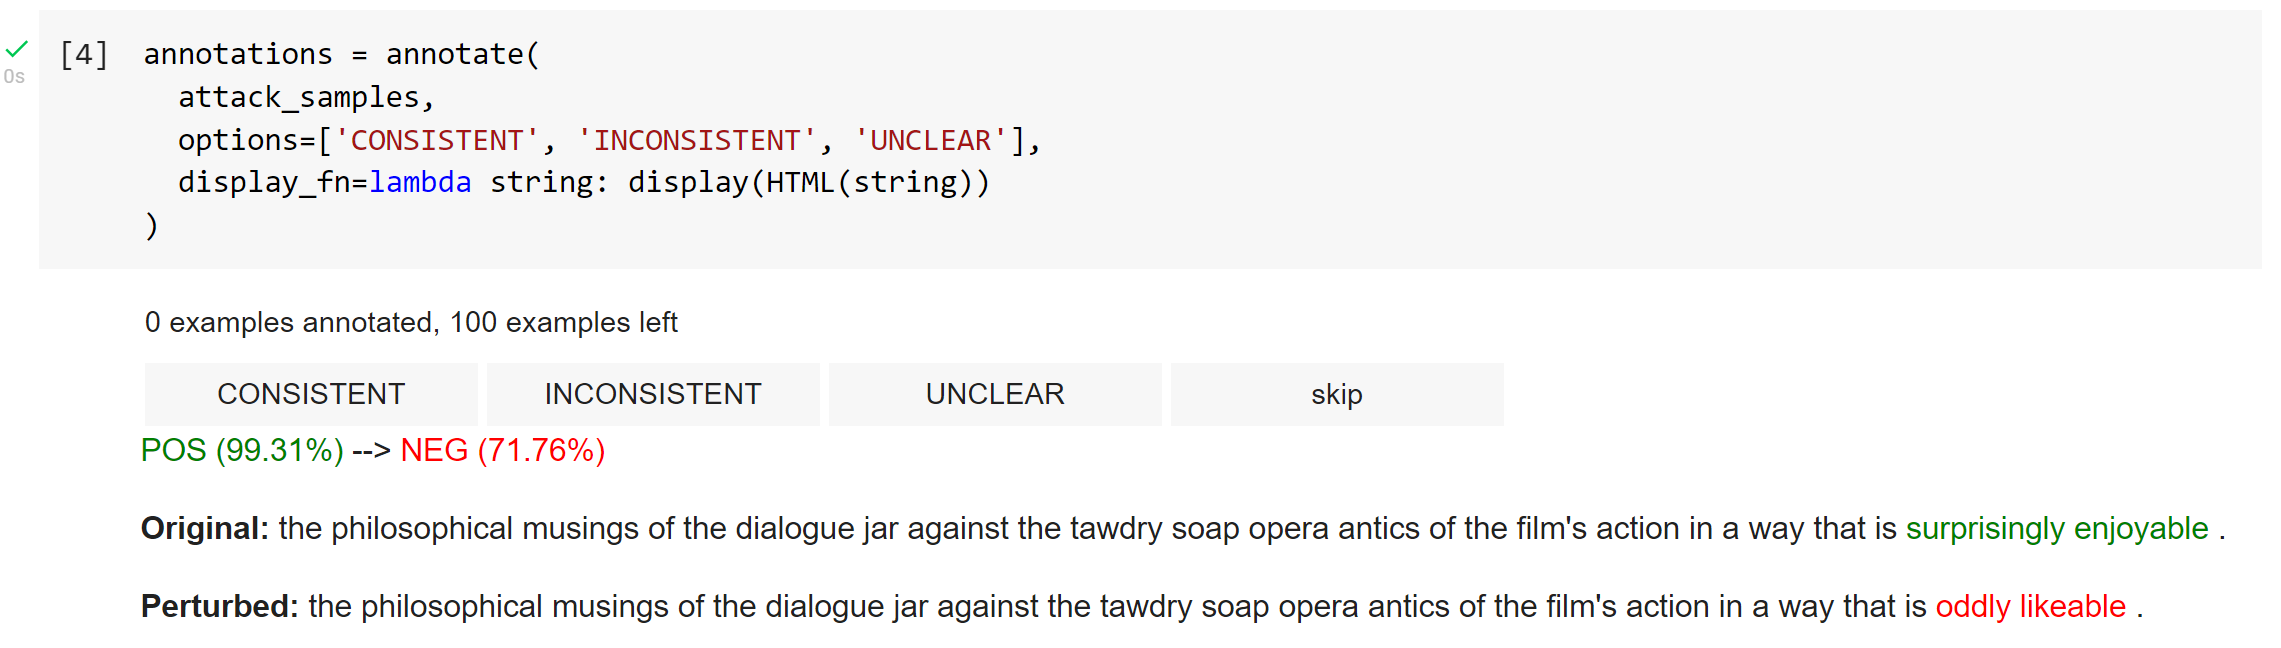
\includegraphics[width=0.99\linewidth]{images/human-evaluation-form.png}
    \caption{Example of the interface used by human judges to evaluate the consistency of the adversarial examples}
    \label{fig:human-evaluation-form}
\end{figure}

We averaged the counts of the adversarial samples based on the labels with which they were annotated. Table \ref{tab:human-evaluation} presents the results of the survey.
The human judgement on BAE confirms the outcome of the contradiction rate metric (see Table \ref{tab:results-rotten}), since more than half of the adversarial examples are inconsistent with the original sample or unclear.
TextFooler instead generates a considerable amount of unclear adversaries (about 17.6\%), meaning that the perturbations frequently end up in sentences that do not make sense.
SynBA seems to be the best attack in terms of human prediction consistency, since it generates only roughly 5\% of inconsistent and 9.3\% of unclear adversarial examples.

To give readers a more detailed insight into the human evaluation, Tables \ref{tab:inconsistent-examples} and \ref{tab:unclear-examples} report some of the adversarial examples annotated as “inconsistent” and “unclear” by all three human judges.

\begin{table}[h]
    \footnotesize
    \centering
    \begin{tabular}{|l|c|c|c|}
        \hline
        \textbf{Label} &            \textbf{TextFooler} &   \textbf{BAE} &    \textbf{SynBA} \\
        \hline \hline
        \emph{Consistent}            &  70.666 &   49.333 &   \textbf{85.666} \\
        \hline
        \emph{Inconsistent}               &  11.666 &   40.666 &  \textbf{5.0}  \\
        \hline
        \emph{Unclear}    &  17.666 &   10.0 &  \textbf{9.333}\\
        \hline
        \end{tabular}
    \caption{Adversarial example counting for labels annotated by human evaluators}
    \label{tab:human-evaluation}
\end{table}


\begin{table}[h]
    \footnotesize
    \centering
    \begin{tabularx}{\textwidth}{|l||X|X|}
    \hline
    \textbf{Method}   &   \textbf{Original}    &   \textbf{Perturbed}\\ \hline\hline
    \emph{TextFooler} & \textcolor{ForestGreen}{POS (99.84\%)}: charlotte \textcolor{ForestGreen}{sometimes} is a gem. it's \textcolor{ForestGreen}{always enthralling}.  & \textcolor{red}{NEG (99.84\%)}: charlotte \textcolor{red}{rarely} is a gem. it's \textcolor{red}{stubbornly puzzling}. \\ \hline
    \emph{BAE} &  \textcolor{ForestGreen}{POS (99.34\%)}: the most \textcolor{ForestGreen}{ingenious} film comedy since being john malkovich  & \textcolor{red}{NEG (99.94\%)}: the most \textcolor{red}{difficult} film comedy since being john malkovich \\ \hline
    \emph{SynBA} & \textcolor{ForestGreen}{POS (99.93\%)}: \textcolor{ForestGreen}{intriguing} and stylish  & \textcolor{red}{NEG (99.66\%)}: \textcolor{red}{puzzling} and stylish  \\ \hline
\end{tabularx}
    \caption{Some adversarial examples annotated as “inconsistent” by human judges}
    \label{tab:inconsistent-examples}
\end{table}

\begin{table}[h]
    \footnotesize
    \centering
    \begin{tabularx}{\textwidth}{|l||X|X|}
    \hline
    \textbf{Method}   &   \textbf{Original}    &   \textbf{Perturbed}\\ \hline\hline
    \emph{TextFooler} & \textcolor{ForestGreen}{POS (99.95\%)}: lan \textcolor{ForestGreen}{yu} is a genuine \textcolor{ForestGreen}{love story} , full of \textcolor{ForestGreen}{traditional layers} of \textcolor{ForestGreen}{awakening} and \textcolor{ForestGreen}{ripening} and \textcolor{ForestGreen}{separation}  &  \textcolor{red}{NEG (76.99\%)}: lan \textcolor{red}{woo} is a genuine \textcolor{red}{affectionate conte} , full of \textcolor{red}{routine grades} of \textcolor{red}{causing} and \textcolor{red}{mature} and \textcolor{red}{seperate} \\ \hline
    \emph{BAE} &  \textcolor{ForestGreen}{POS (99.74\%)}: the \textcolor{ForestGreen}{story} is \textcolor{ForestGreen}{smart} and entirely charming in \textcolor{ForestGreen}{intent} and execution  & \textcolor{red}{NEG (99.88\%)}: the \textcolor{red}{guy} is \textcolor{red}{drunk} and entirely charming in \textcolor{red}{disguise} and execution \\ \hline
    \emph{SynBA} &  \textcolor{red}{NEG (99.87\%)}: even \textcolor{red}{fans} of ismail merchant's work , i suspect , would have a \textcolor{red}{hard} time \textcolor{red}{sitting} through this one &  \textcolor{ForestGreen}{POS (83.9\%)}: even \textcolor{ForestGreen}{amateurs} of ismail merchant's work , i suspect , would have a \textcolor{ForestGreen}{intense} time \textcolor{ForestGreen}{hearing} through this one \\
    \hline
\end{tabularx}
    \caption{Some adversarial examples annotated as “unclear” by human judges}
    \label{tab:unclear-examples}
\end{table}


% from BERT is Robust! A Case Against Synonym-Based Adversarial Examples in Text Classification
% For the human evaluation, we relied on labor crowd-sourced from Amazon Mechanical Turk. 
%We limited our worker pool to workers in the United States and
% the United Kingdom who completed over 5000 Human Intelligence Tasks (HITs)
% with over 98\% success rate. We collected 100 pairs of [original word, attack word]
% for every attack and another 100 pairs for every attack where the context is included with a window size of 11. For the word-pairs, inspired by [24], we asked
% the workers to react to the following claim: “In general, replacing the first word
% with the second word preserves the meaning of the sentence.” For the words with
% context, we presented the two text fragments on top of each other, highlighted
% the changed word, and asked the workers: “In general, the change preserves the
% meaning of the text fragment.” In both cases the workers had seven answers
% to choose from: “Strongly Disagree”, “Disagree”, “Somewhat Disagree”, “Neutral”,
% “Somewhat Agree”, “Agree”, “Strongly Agree”. We convert these answers to a scale
% from 1-7, where higher is better. Every word-pair was judged by ten workers, the
% words with context were scored by five workers each.
%**************************************************************
